\section{\zkwasm\, Architecture Circuits}
\label{chp:architecture-circuits}
\subsection{Setup Circuits}
Setup circuits are filled by the \zkwasm\, compiler component and its purpose is to provide lookup tables $T_\mathcal{C}$, $T_\mathcal{H}$, $T_{module}$ that encode code section, initial memory \& global section and module section.\\

\noindent\emph{Code Section.}
The elementary items in the code section are $opcode$s of instructions that are grouped in a tree like hierarchy. Each instruction can be indexed by $moid$ (modular id), $mmid$ (memory block instance id), $fid$ (function id) and $iid$ (offset of the instruction in a particular function). We denote $iaddr$ tuple of $(moid, mmid, fid, iid)$ and code section can be represented as a map from $iaddr$ to $opcode$. Using the technique in Section \ref{chp:map-repr}, we can encode the code section into $T_\mathcal{C}$ (see Table \ref{tbl:code-table}).

\smallskip\noindent Code table $T_\mathcal{C}$ is later used to constrain entries in memory execution table $T_\mathcal{E}$ (see Section \ref{chp:ex-table}) such that if $e \in T_\mathcal{E}$ then $(e.iaddr, e.opcode)$ must also in $T_\mathcal{C}$. 

\begin{table}[!h]
\begin{center}
\begin{tabular}{ | c | c | c | c | c | }
  \hline
  moid & mmid & fid & iid & opcode \\ 
  \hline
\end{tabular}
\caption{execution table}
\label{tbl:code-table}
\end{center}
\end{table}

\noindent\emph{Initial Memory \& Global Section.}
The element items in the memory section of WASM image are unsigned 64 bit words (u64). The address of each $u64$ word can be indexed by $mmid$ and $offset$. Besides the value, memory can have types that are either mutable of immutable. Thus the memory section can be represented as a map from $(mmid, offset)$ to $(value, isMutable)$. Similarly, using the technique in Section \ref{chp:map-repr}, we can encode the initial memory section into $T_\mathcal{H}$. According to WASM specification, global objects represent variable instances that can be shared between different modules. Since the access model of memory and global objects are similar, we merge two tables into one and use $ltype = Memory \,|\, Global$ to distinguish them (see Table \ref{tbl:init-memory-table}).
\begin{table}[!h]
\begin{center}
\begin{tabular}{ | c | c | c | c | c | }
  \hline
  $ltype$ & $mmid$ & \emph{offset} & $value$ & $isMutable$ \\
  \hline
  $Heap$ & $mmid_0$ & $1$ & $0x01$ & $true$ \\
  \hline
  $Heap$ & $mmid_1$ & $1$ & $0x01$ & $true$ \\
  \hline
  $Global$ & $mmid_2$ & $1$ & $0x01$ & $true$ \\ 
  \hline
  $Global$ & $mmid_3$ & $1$ & $0x01$ & $false$ \\ 
  \hline
\end{tabular}
\caption{initial memory table}
\label{tbl:init-memory-table}
\end{center}
\end{table}

We use $T_\mathcal{H}$ to constrain entries in the memory access log table $T_\mathcal{M}$ (see Table \ref{tbl:rw-table}) so that $\forall e, e\in T_\mathcal{M} \wedge e.accessType = Init \rightarrow (e.iaddr, value) \in T_\mathcal{H}$.


\subsection{Execution Trace Circuits.}
\label{chp:ex-table}
Execution Trace Circuits are derived from the execution trace emulated from WASMI (WASM intepreter). Each trace element is related to an instruction in the code table $T_\mathcal{C}$ and has a predefined semantic based on the opcode. To define the semantics of a WASM op, we use three steps. First, since WASM is a stack machine, we define the \emph{operands} of an opcode $op$ to be
\[
operands(op) = p_0, p_1, p_2 \cdots, p_k
\]
where $p_i$ are values on the stack and $p_i = stack[sp+i]$.
Second, we define the semantics of $op$ by a sequence of micro operations
\[
mop_i = \begin{cases}
    w_i = load(ltype, addr)\, \textnormal{ where $addr \in \{p_1, p_2, \cdots, p_k, w_0, w_1, \cdots, w_{i-1}\}$}\\
    write(ltype, addr, v)\, \textnormal{ where $addr, v \in \{p_1, p_2, \cdots, p_k, w_0, w_1, \cdots, w_{i-1}\}$}\\
    w_i = arith(p_1, p_2,\cdots, p_k, w_0, w_1); \\
    \textit{FALLTHOUGH}; \\
    GOTO(iaddr); \\
    if \, b\, then\, \{mop_{i+1}, \cdots mop_{j}\} \,else\, \{mop_{j+1},\cdots\}.
    \end{cases}
\]
When writing execution trace into the execution circuit, we arrange the instruction into small blocks of the execution circuit such that each block represents an instruction. Within each block, we use the $start$ column to indicate whether this row is the start of a new instruction block and put $op$ and $mop$ in the opcode column. In the address column, we push all used addresses and the first row is the instruction address of this instruction in $T_\mathcal{C}$ and in the $sp$ column we record all the sp changes.
\begin{table}[!h]
\begin{center}
\begin{tabular}{ | c | c | c | c | c | c | c | c | c | c | c | }
  \hline
  start & opcode & bit cell & state & aux & $address \in T_{I}$ & $sp \in T_\mathcal{F}$& u64 cell & operand \\ 
  \hline
   true & $op$ & $b_0$ & $s_0$ & $aux$ & $iaddr_0$ & sp & $w_0$ & $bop$\\ 
 \hline
   0 & $mop_0$ & $b_1$ & $s_1$ & $aux_0$ & $addr_0$ & sp & $w_1$ & $bop$\\ 
 \hline
   0 & $mop_1$ & $b_2$ & $s_2$ & $aux_1$ & $addr_1$ & sp & $w_2$ & $bop$\\ 
 \hline 
  0 & $mop_2$ & $b_3$ & $s_3$ & $aux_2$ & $addr_2$ & sp & $w_3$ & $bop$\\ 
 \hline
   $\cdots$ & $\cdots$ & $\cdots$ & $\cdots$ & $\cdots$ & $\cdots$ & $\cdots$ & $\cdots$ & $\cdots$\\ 
 \hline
   true & $op_1$ & $b$ & $s$ & $aux$ & $iaddr_1$ & sp & $w$ & $bop$\\ 
 \hline
   $\cdots$ & $\cdots$ & $\cdots$ & $\cdots$ & $\cdots$ & $\cdots$ & $\cdots$ & $\cdots$ & $\cdots$\\
 \hline
 \hline
\end{tabular}
\caption{execution table}
\label{tbl:ex-table}
\end{center}
\end{table}

Although different opcodes might have different semantics thus different $mop_k$, $addr_i$, etc. There are some common constraints that we need to enforce in the execution circuit.

First. we need to enforce that each instruction exists in the code section, thus $(iaddr, opcode) \in T_\mathcal{C}$. Second, suppose that $operand$ $p_i$ is got from stack pointer $sp$ as a result of $mop_k(sp)$, then $(sp, read, iaddr, k, p_i) \in T_{\mathcal{M}}$, which means the result $p_i$ is enforced from a valid memory access log table. Similarly, suppose that witness $w_i$ is got from memory access of $addr_j$ with access type $ltype$ as a result of $mop_k$, then $(mem, addr_j, ltype, k, w_i) \in T_{\mathcal{M}}$.  Third, we enforce that all the cells in bit column are either zero or one and all the cells in u64 witness column and operand column are in $T_64$ (less than $2^{64}$).
\subsection{Access Log Circuit}
\label{chp:access-log-circuit}
Recall that the access log circuit is a unique table corresponding to a valid memory access log sequence and satisfies Equation \ref{eq:rw-constraints}. In WASM specification, an access log is used for three different types that are memory access, stack access and global access. Each access log can be one of the three types: \emph{Init}, \emph{Read} or \emph{Write} and all logs are sorted by $(addres, (tid, tmid))$ where $address$ is indexed by $ (mmid, offset)$, $tid$ is the transition index of the execution log that contains the access and $tmid$ is the index of the access micro-op in that instruction.

\begin{table}[!h]
\begin{center}
\begin{tabular}{ | c | c | c | c | c | c | c | c |}
  \hline
  section & ltype & mmid & offset & tid & emid & value\\ 
  \hline
  memory | stack | global & \emph{Init} | Read | Write & & & & &\\
 \hline
\end{tabular}
\caption{access log circuit}
\label{tbl: rw-circuit}
\end{center}
\end{table}

\subsection{Frame Circuit}
\label{chp:frame-circuit}
Frame entry is a tuple of $(tid, frameTid, iaddr)$. 
frameId is the tid in which instruction has called semantic. 
\subsection{Support Zero-knowledge in IO}
Zero-knowledge of inputs is not supported in WASM specification. Thus to support the private inputs that we do not want to leak, we add special instructions in the \zkwasm, virtual machine which are \emph{get\_private\_input} and \emph{get\_public\_input} for input and \emph{put} for output. We represent public inputs in a separate column and use polynomial lookup to link input values with the result of \emph{get\_private\_input(inputCursor)} (See Figure \ref{fig:public-input}).

\begin{figure}[!ht]
\centerline{
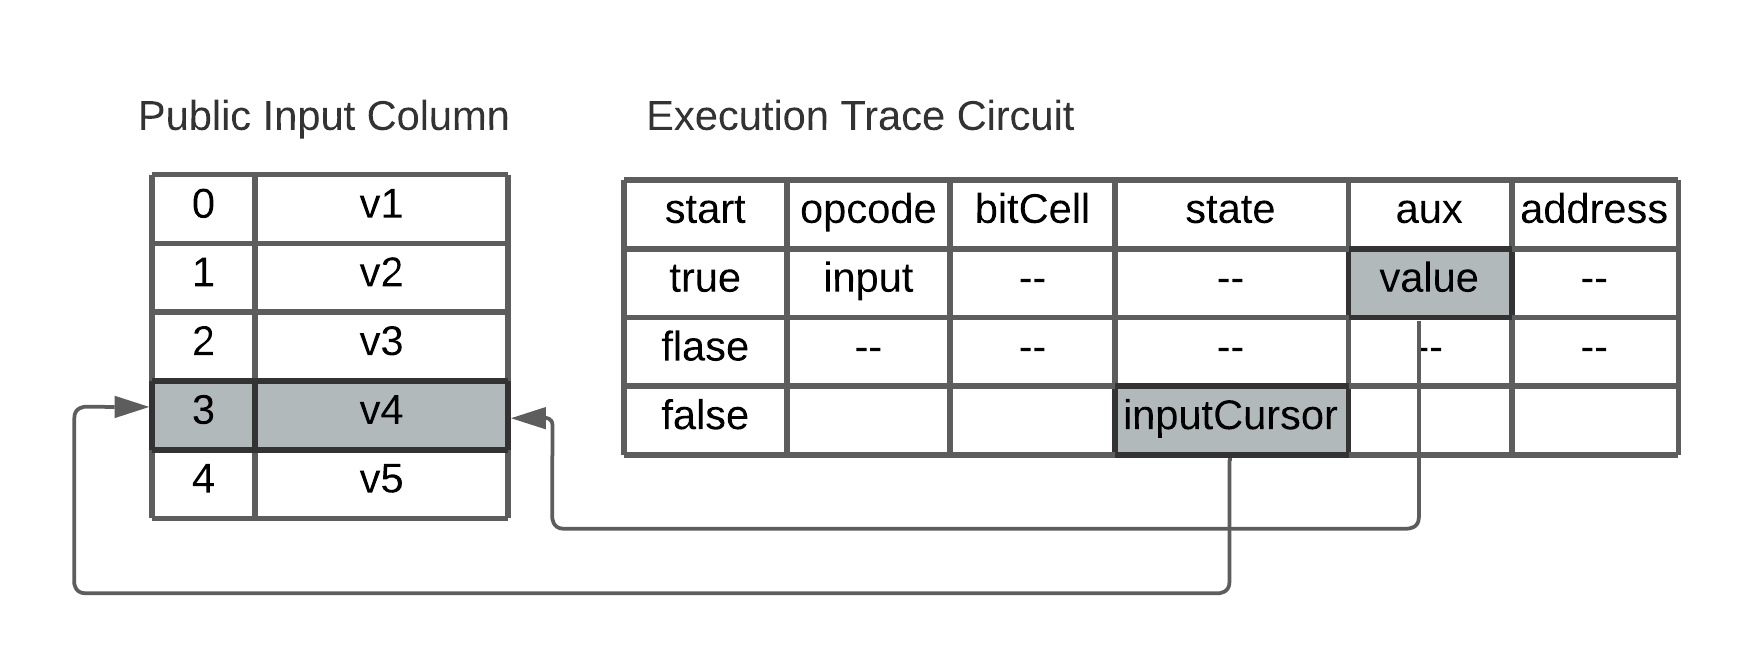
\includegraphics[scale=0.8]{figs/public-input.png}
}
\caption{Public Input Circuit}\label{fig:public-input}
\end{figure}
 Similarly we use a separate column to hold output data and use a polynomial lookup to enforce that the value we output in the execution circuit aux cell is the same as in the output column. When dealing with private inputs, we can put them into the stack with no constraints. (why)